\documentclass[11pt]
{article}
\usepackage{graphicx}
\usepackage{subcaption}
\usepackage{float}
\usepackage{hyperref}
\usepackage[bottom]{footmisc}
\usepackage{babel}[English]
\usepackage{apacite}

\title{DL LAB 2: An application with RNN}
\author{Senne Deproost and Diego Saby}
\date{November 2019}


\begin{document}
\maketitle
\section{Introduction}
In the field of machine learning we try create computational models to find solutions for a wide set of tasks. One of the more popular problems to solve are the classification of instances and function approximation with regression. Solutions like \textit{Support Vector Machines} and \textit{Decision Trees} have already proven their worth in the past. Techniques from the deep learning (DL) sub-field of machine learning have shown their usability when tackling on data with high dimen\-sionality. Deep learning's ability to scale better with these kinds of data makes it useful in many application domains like machine control and decision support systems. Variations in the model's architecture could insure better performance on a domain specific task.\\

One DL architecture we'll focus on in this lab report is the \textit{Recurrent Neural Network} architecture. Whereas classical \textit{Feedforward Neural Network} (FNN) only allows the passage of activation through the neuron layers, a RNN network will remember the neuron activations from a previous step in time. This is implemented with the inclusion of memory nodes that will hold on to previous encountered activation values. An advantage of this kind of networks is the usage of \textit{Temporal Sequences}, allowing the model to train on data like text sentences, music recordings and streams of data.\\

Automated content creation using DL models has known a significant rise in popularity over the past years. With \textit{Generative Adverserial Networks} (GAN's), we can use two competing networks to train a generator for images \cite{Goodfellow2014}. In this architecture, one network, the has to mimic given image data input distribution and another adversarial network that has to estimate the loss of the predicted regression with given training data. This prediction can then be used to optimize the generative network. Other types of models like \textit{transformers}, recently used in OpenAI's GPT-2 model \cite{Radford}, can generate human-like text paragraphs with the potential of passing the famous Turing test. With a rise in the exploration of the generative content field, researches already used RNN based models to generate content like images \cite{Gregor}, voice synthesis \cite{Oord2016,VanDenOord2016} and music \cite{Oord2016}.\\

Music generation can be seen as a series of notes. We can try to predict the next note given the previous series of notes.
For this kind of problem RNNs are useful.

\subsection{Problem}
In this report, we will focus on three types of models in the task of creating music from MIDI files. The data will consists of fragments of Chopin's Nocturne music composition in the MIDI file format with 30 available notes available on the tone ladder. The music consists of only one music instrument: the piano.

Apart from regular RNNs, we will experiment on \textit{Long Short-Term Memory} (LSTM)\cite{Hochreiter:1997:LSM:1246443.1246450} and \textit{Gated Recurrent Unit } (GRU) models \cite{Cho}.

\subsection{LSTM}
An LSTM is a form of RNN which solves the problem of the large decay in loss function gradient over long periods of time. Specialized memory cells are used to recall on several past activations for longer periods of time. In addition, the network contains gates to control the information flow to and from memory and when it can be returned to its initial status.

\subsection{GRU}
GRU are similar in construction to LSTM that they have gates to control the specialized memory cells. However, these models are simplified containing less gates and dont make the distinction between memory cells and normal ones \cite{Chung}.

\begin{figure}[H]
	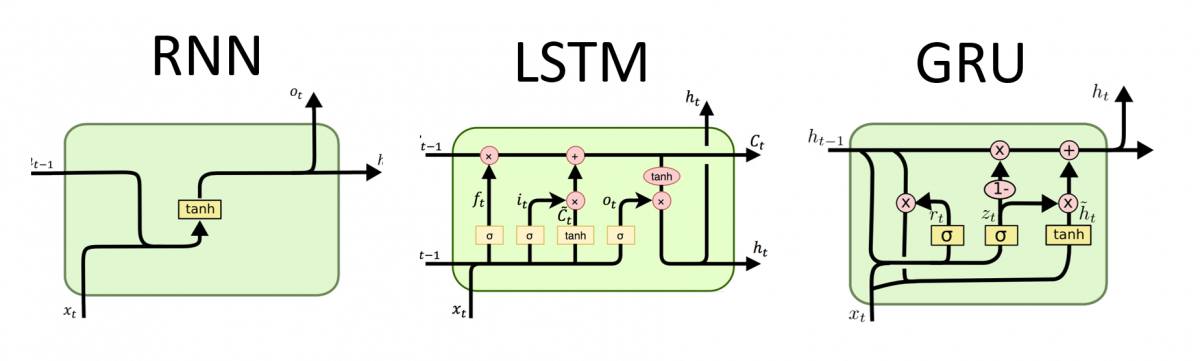
\includegraphics[width=\linewidth]{comp.png}
	\caption{An overview of the three kinds of models used in the experiments. Left we have a simple RNN node containing a simple $tanh$ activation function. In the middle the internal gates of the LSTM node are shown. The right contains the simplified layout of a GRU network node.}
	\label{fig:fig1}
\end{figure}


%\begin{itemize}
%	\item talk about RNN and LSTM
%	\item Talk about how RNN is useful for music
%	\item Introduce our project -> RNN on Chopin Nocturnes
%	\item Something else?...
%\end{itemize}


\section{Preprocess the data}
One of the first questions we were opposed to was how to encode music in order to train the Neural Network. Our source files are midi files. They are an useful way to encode the music where we can extract the notes and their duration from the file.\\
To simplify the problem we decided to abstract the notes duration and just use the notes pitch. \\
\subsection{Enumerating the notes}
Our first attempt was done inspired by some code found on the internet to produce video games music. \textbf{add reference}\\
To extract the notes the notes from midi file we used a library called \textit{Music21}. It provided us with the notes names or chord names that were played. From there we have a sequence of notes names. Then we just assign the notes a number.
For the prediction we used a vector of all the notes and a with 1 for the next note that follows the sequence and 0 for the others.\\
After several experiments using a as the last layer a Fully connected NN with a \textit{softmax} activation function and taking the note with the biggest probability to be the next one as the prediction of the next note, the results were disappointing. No matter what was the input it always yielded the same note. After changing the RNN architecture, the learning rate, the optimization function, it changed the note that was predicted, but always was a sequence of the same  note.

\section{Experiments}
In the experiments, we mainly focus on the three different kind of models as described before. We first vary the numbers of node in the hidden layers of the network. Afterwards, we change the number of layers in the network. We train with a fixed batch size of 64 during a 200 epoch session. The results will be discussed based upon the loss function of the model and the qualitative analysis of the generated music fragments. We fixed the window lag of notes to 30 notes, to predict the next one, and we did not put any skipping to generate the data training.


\subsection{Vanilla RNN}
\subsection{LSTM}
\subsection{GRU}
Last we run experiments with the GRU variant of RNN's. 

\subsubsection{Number of nodes}
\subsubsection{Number of layers}




\section{Conclusion}


\bibliographystyle{apacite}
\bibliography{references}

\end{document}